\documentclass[a4paper,11pt,fleqn]{article}%fleqn pour aligner les equations à gauche
\usepackage{../../Styles/Eval}

\newcommand{\chnum}{DS5 - B}
\newcommand{\chtitle}{DS 5 : Ondes et Cinétique chimique}
\newcommand{\dtype}{DS}

\begin{document}
	\maketitle

\section{Etude cinétique d’une réaction d’oxydoréduction}
On se propose d’étudier la cinétique de la transformation lente de décomposition de l’eau oxygénée par les ions iodure en présence d’acide sulfurique, transformation considérée comme totale.\\
L’équation de la réaction qui modélise la transformation d’oxydoréduction s’écrit :
\\
\ce{H2O2(aq) + 2 I-(aq) + 2 H+(aq) <=> I2(aq) + 2H2O(l)}\\

La solution de diiode formée étant colorée, la transformation est suivie par spectrophotométrie, méthode qui consiste  à mesurer l'absorbance A de la solution, grandeur proportionnelle à la concentration en diiode.

	\subsection{Étude théorique de la réaction}
	\begin{enumerate}
		\item Identifier,  dans l'équation de la réaction étudiée, les deux couples d'oxydoréduction mis en jeu en écrivant leurs demi-équations correspondantes.
		Justifier l’écriture de l’équation de la réaction.
	\end{enumerate}
	\subsection{Suivi de la réaction}
	À la date $t$= \SI{0}{s}, on mélange un volume $V_1$ = \SI{20,0}{mL} d'une solution d'iodure de potassium (\ce{K+} ; \ce{I-}) de concentration $C_1$ = \SI{2,0}{mL} d'eau oxygénée \ce{H2O2} de concentration$C_2$ = \SI{0,10}{\mole\per\liter}.\\
	On remplit une cuve de spectrophotométrie et on relève les valeurs de l'absorbance au cours du temps. On détermine alors, grâce à la loi de Beer-Lambert, la concentration en quantité de matière  [\ce{I2}] du diiode formé :\\
	\begin{tabular}{|c|c|c|c|c|c|c|c|}
		\hline t (s)& 0 & 126 & 434 & 682 & 930 & 1178 & 1420\\
		\hline [\ce{I2}] (\unit{\milli\mole\per\liter}) & 0,00 & 1,74 & 4,06 & 5,16 & 5,84 & 6,26 & 6,53\\
		\hline
	\end{tabular}
	
	\begin{enumerate}
		\item Justifier l'utilisation du spectrophotomètre pour le suivi cinétique de la réaction.
		\item Rappeler la relation entre l'absorbance $A$ et la concentration en quantité de matière [\ce{I2}] de l'espèce colorée.
		\item Le mélange initial est-il dans les proportions sot\oe chiométriques ? Justifier la réponse par des calculs.
		\item Compléter le tableau d'avancement de la transformation et justifier les calculs de $n_1$ et $n_2$.\\
		\noindent \begin{tabular}{|>{\centering}m{3cm}|>{\centering}m{2cm}|>{\centering}m{2cm}|>{\centering}m{2cm}|>{\centering}m{2cm}||>{\centering}m{2cm}|>{\centering\arraybackslash}m{2cm}|}
			\hline
			\multicolumn{2}{|c|}{Équation chimique} & \multicolumn{5}{|c|}{\ce{H2O2(aq) + 2 I-(aq) + 2 H+(aq) <=> I2(aq) + 2H2O(l)}}\\
			\hline État du système & Avancement (\unit{\mole}) & \multicolumn{5}{|c|}{Quantité de matière (\unit{\mole})}\\
			\hline État initial & 0 & $n_2$ = \num{2,0e-4} & $n_1$ = \num{20e-4} & Excès & Beaucoup & \\
			\hline État en cours de transformation & $x$ & & & Excès & Beaucoup & \\
			\hline État final & $x_{max}$ & & & Excès & Beaucoup & \\
			\hline
		\end{tabular}
		\item Déterminer l'avancement maximal. En déduire la valeur théorique de la concentration en diiode formé lorsque la transformation est terminée. Cette concentration est-elle en accord avec le tableau de mesures ?
	\end{enumerate}
	
	\subsection{Exploitation des résultats}
	À l'aide d'un tableur, on calcule la concentration et la vitesse de disparition de l'eau oxygénée au cours du temps. Une capture d'écran est donnée ci-dessous.\\
	\begin{center}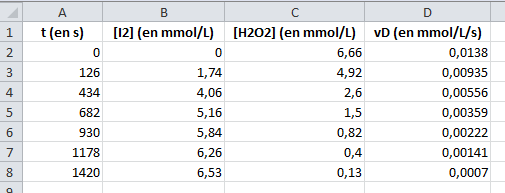
\includegraphics[scale = .5]{Ressources/TSPE_C10_Eval_Fig8.png}\end{center}
	\begin{enumerate}
		\item Donner la définition du temps de demi-réaction dans le cas étudié, puis déterminer graphiquement $t_{1/2}$ à l'aide de la courbe de l'évolution de la concentration en eau oxygénée au cours du temps ci-après.\\
		\begin{center}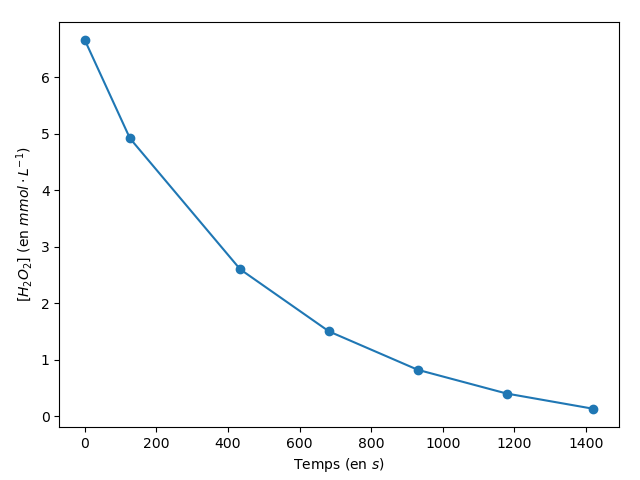
\includegraphics[scale = .8]{Ressources/TSPE_C10_Eval_Fig6.png}\end{center}
		\item  Retrouver par un calcul, la vitesse de disparition de \ce{H2O2} à $t$ = \SI{434}{s}.\\
		On trace ensuite la courbe donnant la vitesse de disparition $v_D$ de l'eau oxygénée en fonction de sa concentration.\\
		\begin{center}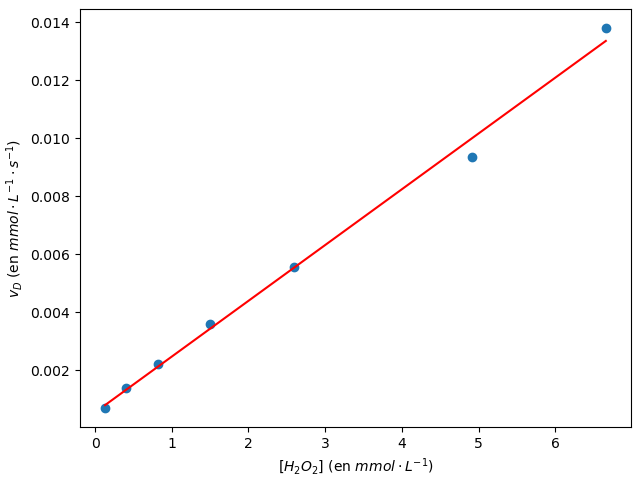
\includegraphics[scale = .7]{Ressources/TSPE_C10_Eval_Fig7.png}\end{center}
		\item Expliquer pourquoi cette transformation chimique suit une loi de vitesse d'ordre 1.
		\item La modélisation de la concentration en eau oxygénée au cours du temps est donnée par la relation :\\ $[\ce{H2O2}](t) = [\ce{H2O2}]_0 \cdot  e^{-kt}$\\
		À l'aide de cette relation et du tableau de mesures, déterminer [\ce{H2O2}]$_0$, concentration initiale en eau oxygénée.
		\item Retrouver cette valeur par le calcul.
		\item Déterminer $k$ la constante de vitesse en utilisant la droite donnant la vitesse de disparition $v_D$ de l'eau oxygénée en fonction de sa concentration.
	\end{enumerate}
\section{Profil d'une figure de diffraction}
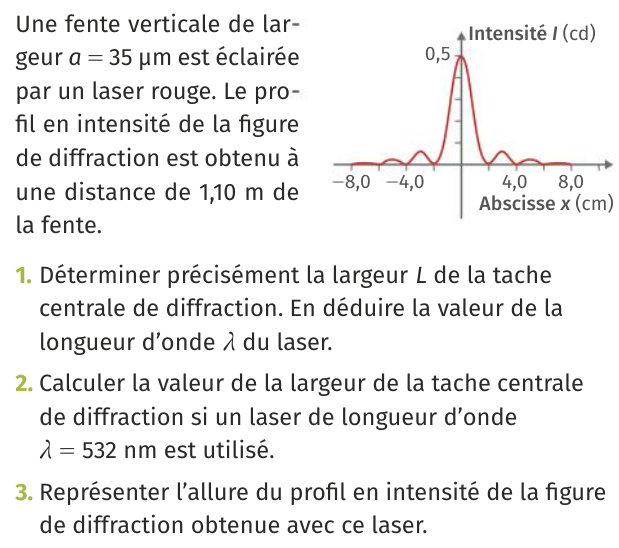
\includegraphics[scale=.5]{Ressources/TSPE_C10_Eval_Fig9.png}
\end{document}